\subsection[EUPHONY]{EUPHONY:~unification of malware labels}

\begin{frame}
    \frametitle{Why do we need to unify malware labels?}
    \centering

    We cannot access antivirus descriptions with simple techniques

    \vspace{-10pt}

    \begin{table}[!ht]
        \resizebox{\textwidth}{!}{
            \textit{
                \begin{tabular}{ c c }
    Monitoring-Tool:Android/AccuTrack.beta & Android/Tracker.A!tr \\ 
    Trojan-Spy.AndroidOS.AccuTrack.a & Android.Spyware.AccuTracker.1 \\ 
\end{tabular}

            }
        }
    \end{table}

    \vspace{-10pt}

    \begin{figure}[!ht]
        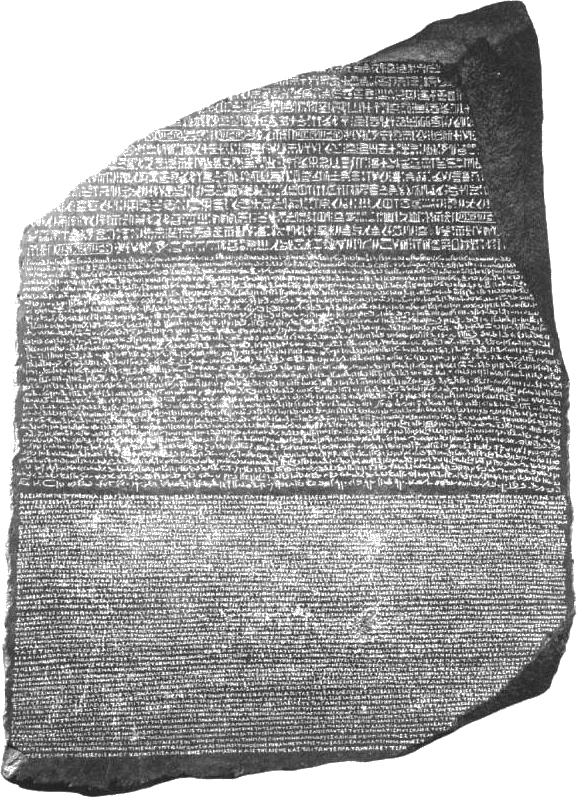
\includegraphics[height=0.65\textheight]{figures/euphony/rosette.png}
    \end{figure}

\end{frame}

\begin{frame}
    \vfill
    \centering
    \usebeamerfont{title}

    \begin{beamercolorbox}[sep=8pt,center,shadow=true,rounded=true]{title}
        \textbf{EUPHONY}:\\
        unification of malware labels

        \small{}

        \bigskip{}

        \textit{
            Euphony: Harmonious Unification of Cacophonous \\
            Anti-Virus Vendor Labels for Android Malware}

        \medskip{}

        The 14th International Conference on \\
        Mining Software Repositories (MSR)
    \end{beamercolorbox}

    \vfill
\end{frame}

\begin{frame}
    \frametitle{Reminders and methodology}

    \begin{columns}
        \begin{column}{0.3\textwidth}
            \begin{figure}[!ht]
                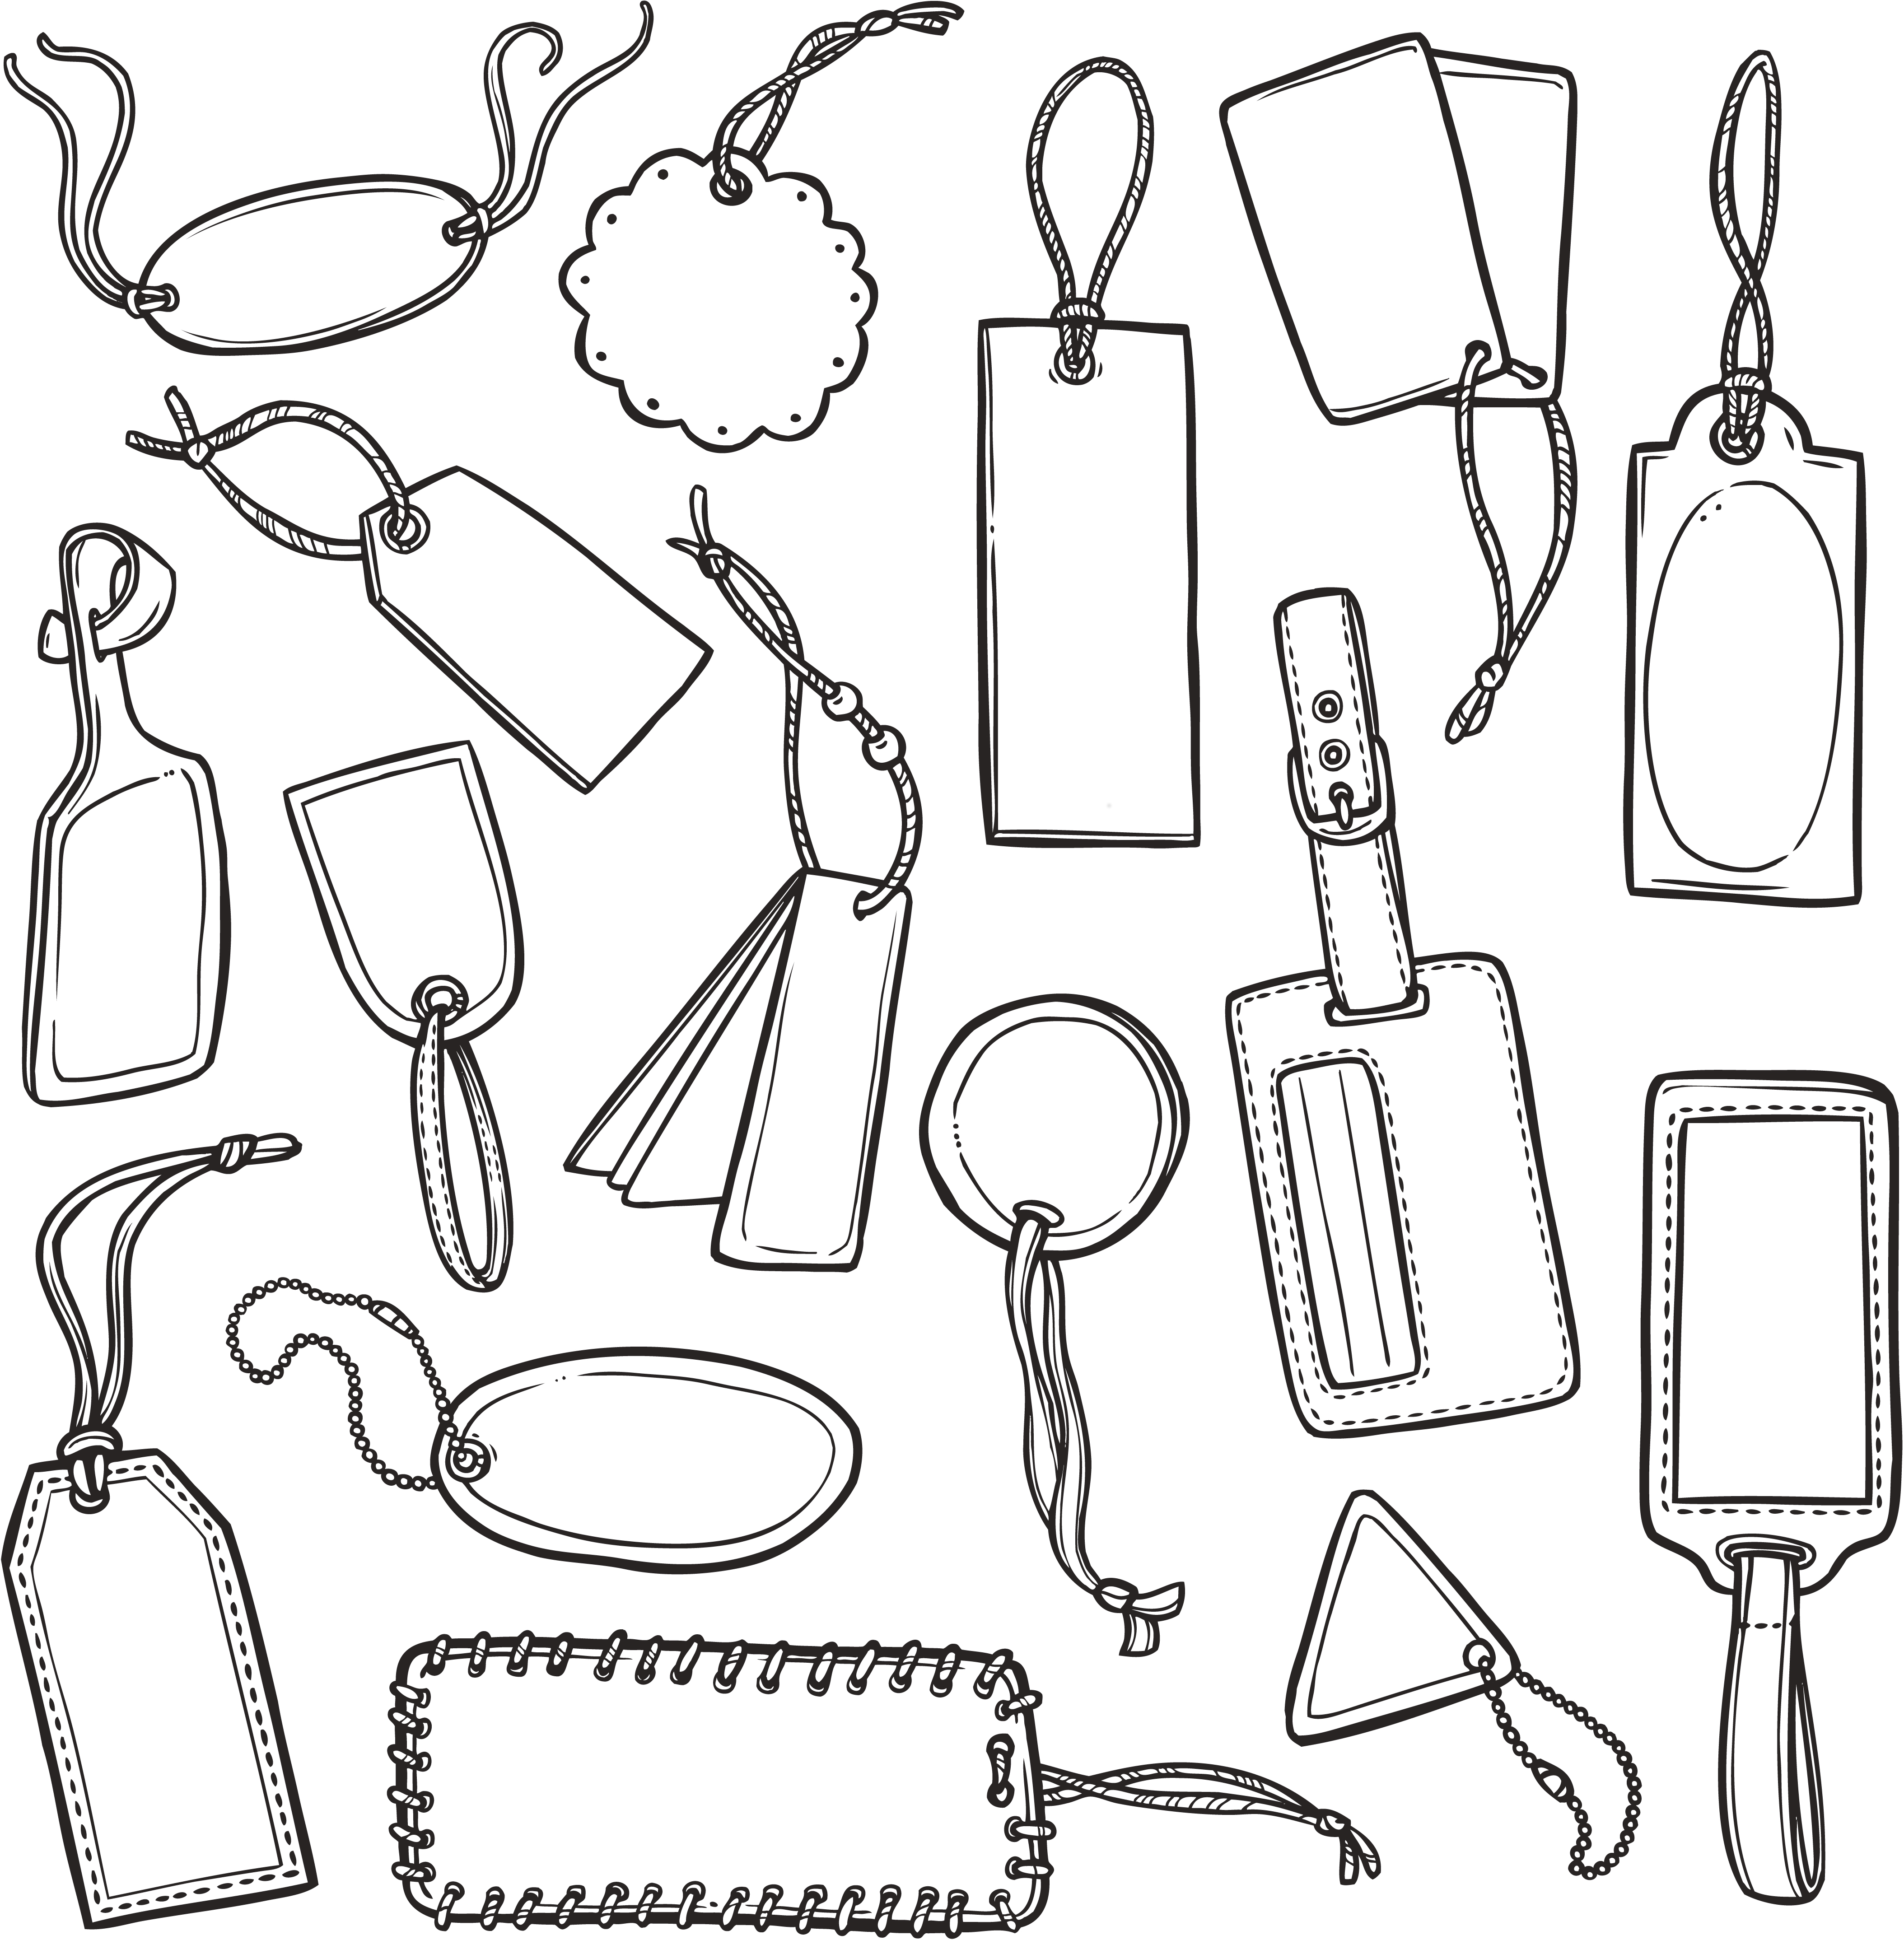
\includegraphics[width=0.95\textwidth]{figures/euphony/tag.jpg}
            \end{figure}
        \end{column}

        \begin{column}{0.81\textwidth}
            \begin{block}{}
                \centering
                \textbf{Reminders}
            \end{block}
            \begin{itemize}
                \item Antivirus help experts to create ground truths
                \begin{itemize}
                    \item e.g., type, family, platform, information \ldots
                \end{itemize}
                \item But labels include syntactic and semantic errors
                \item How to retrieve the words embedded in labels?
            \end{itemize}

            \begin{block}{}
                \centering
                \textbf{Methodology}
            \end{block}
            \begin{itemize}
                \item Develop a program to parse and cluster labels
                \item Compare our approach against state-of-the-art
                \item Investigate the label families retrieved from:
                \begin{itemize}
                    \item Genome, Drebin, and Androzoo datasets
                \end{itemize}
            \end{itemize}
        \end{column}
    \end{columns}

\end{frame}

\begin{frame}
    \frametitle{Input and Output}

    \begin{figure}
        \vspace{-5pt}
        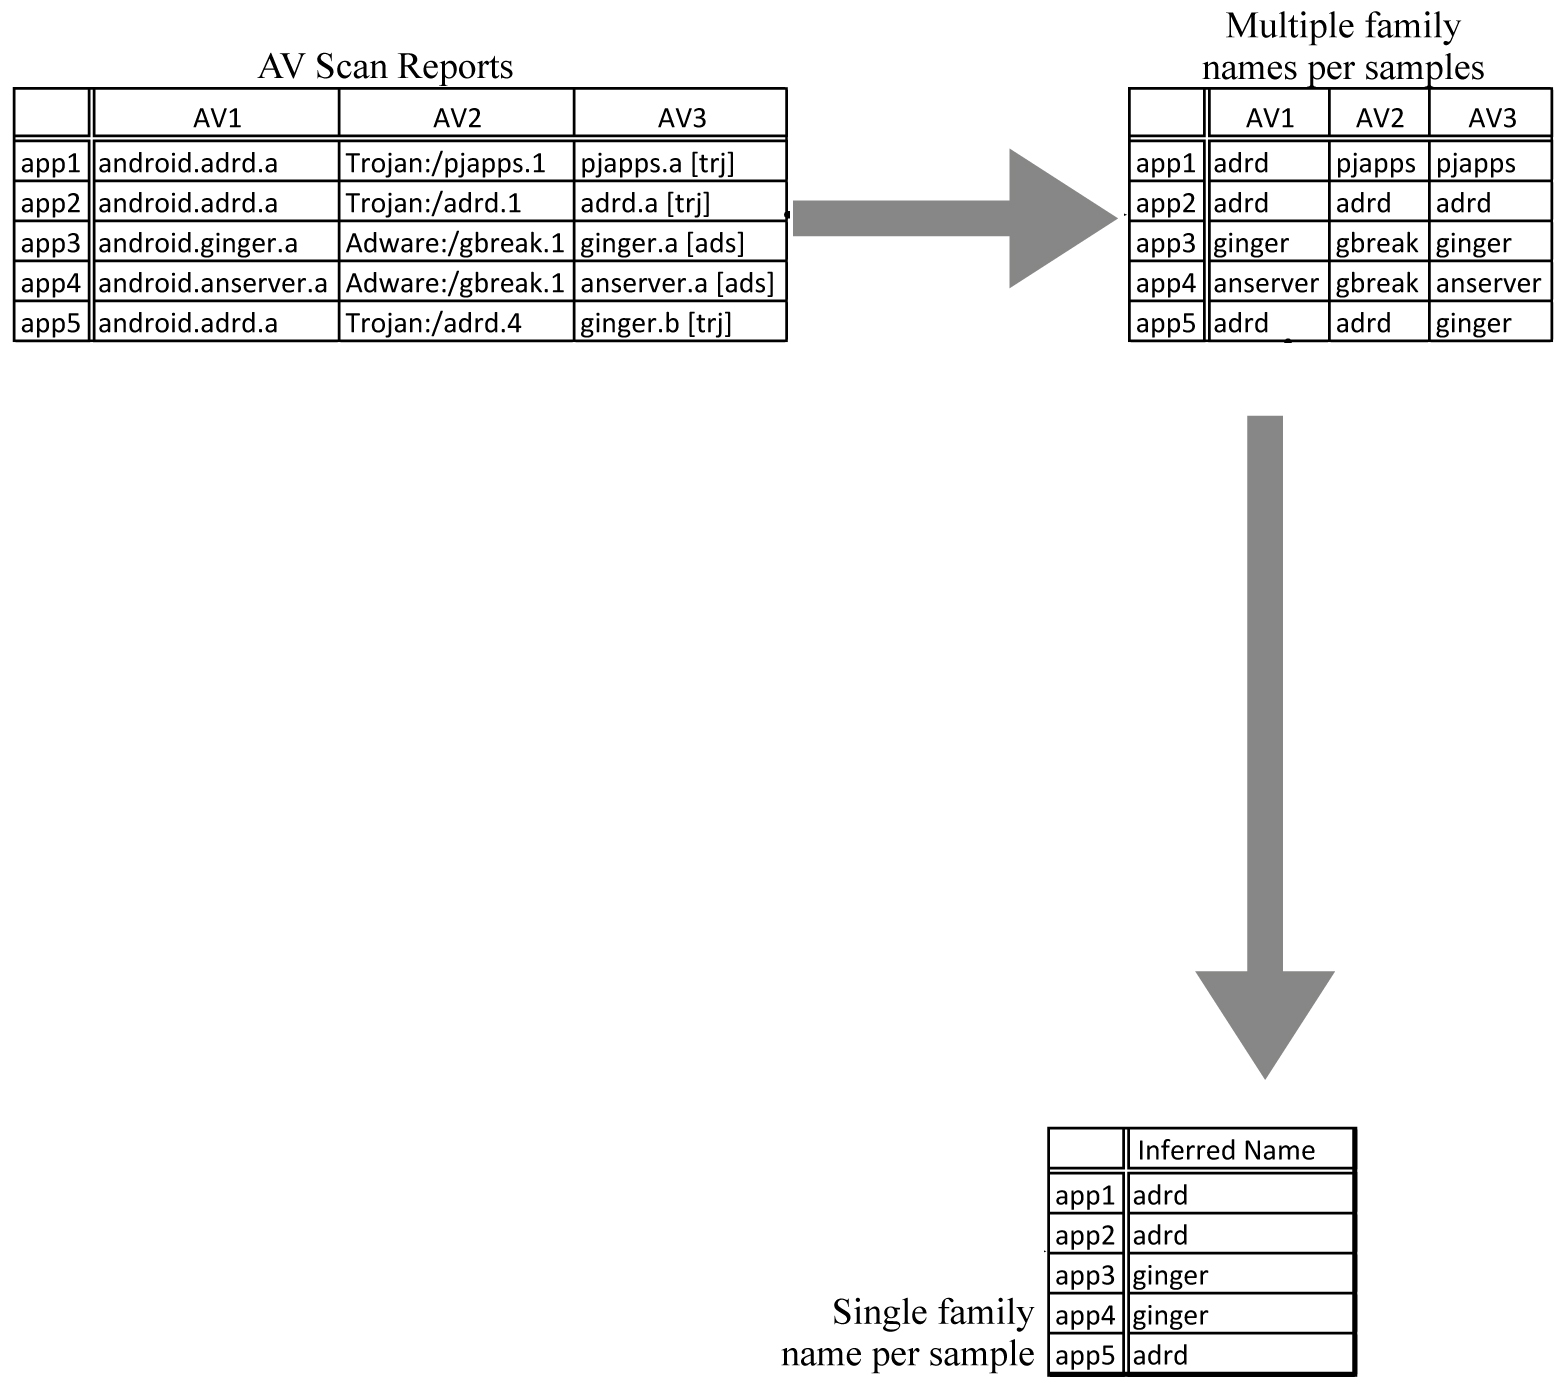
\includegraphics[width=0.8\textwidth]{figures/euphony/architecture-zero.jpg}
    \end{figure}

\end{frame}

\begin{frame}
    \frametitle{EUPHONY architecture}

    \begin{figure}
        \vspace{-5pt}
        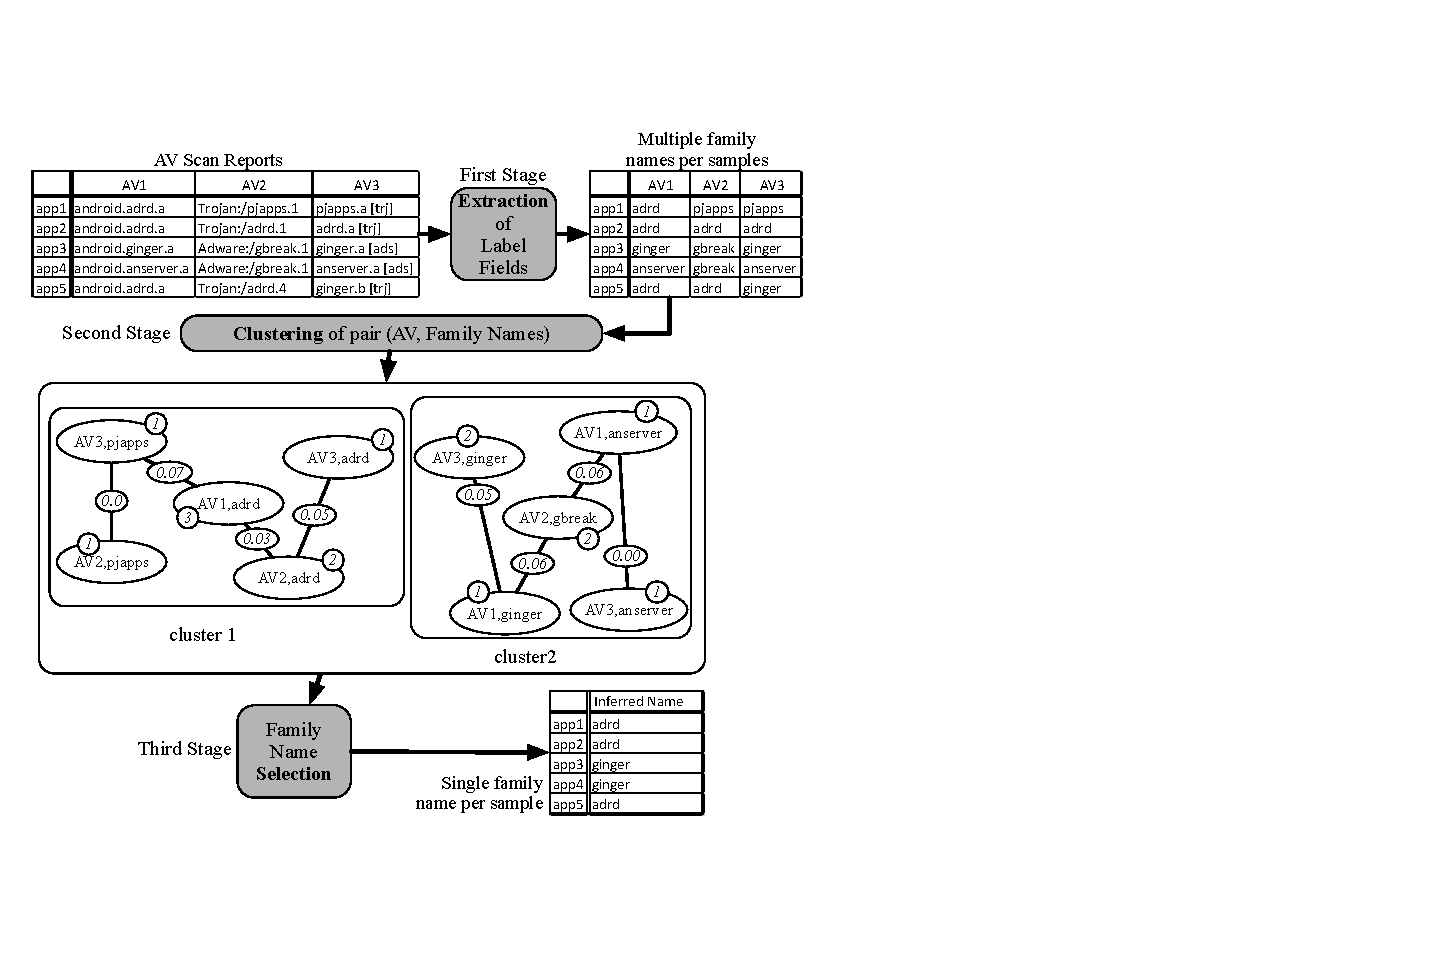
\includegraphics[width=0.8\textwidth]{figures/euphony/architecture.pdf}
    \end{figure}

\end{frame}

\begin{frame}
    \frametitle{EUPHONY architecture}

    \begin{figure}
        \vspace{-5pt}
        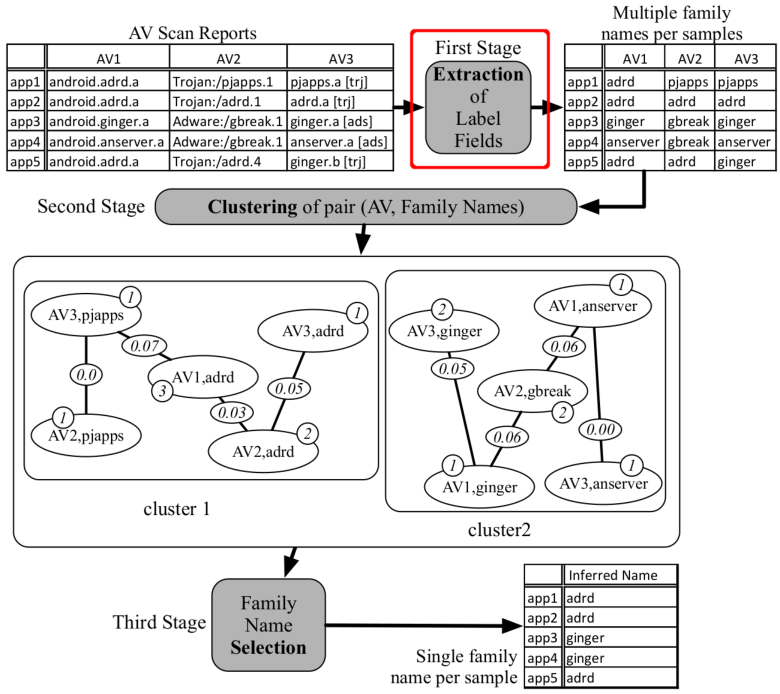
\includegraphics[width=0.8\textwidth]{figures/euphony/architecture-first.pdf}
    \end{figure}

\end{frame}

\begin{frame}
    \frametitle{Stage 1: extraction of label fields}
    \centering
    \begin{figure}[!ht]
        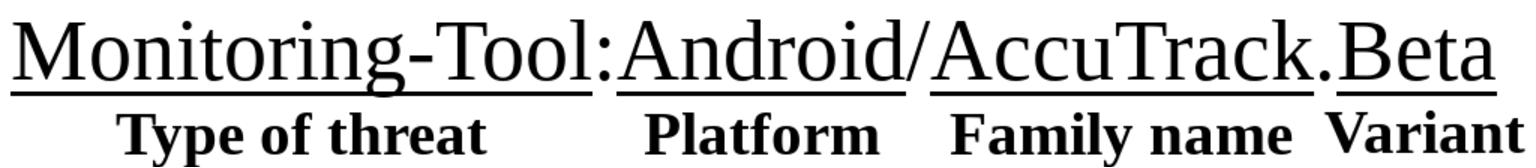
\includegraphics[width=0.7\textwidth]{figures/euphony/label.pdf}
    \end{figure}

    \vspace{-20pt}

    \begin{columns}
        \begin{column}{0.6\textwidth}
            \begin{algorithm}[H]
                \tiny
                \begin{algorithmic}[1]
    \State $Mapping \gets [name, type, platform, information]$
    \Function{Parse}{$knowledge_{db}$, $heuristics$, $labels$}
    \State $mappings \gets \Call{map}{Mapping, labels}$
    \State $pqueue \gets \Call{prio-queue}{mappings}$
    \While{\Call{not-empty?}{$pqueue$}}
    \State $m \gets \Call{peek}{pqueue}$
    \For{$H$ in $heuristics$}
    \State $findings \gets \Call{h}{knowledge_{db}, m}$
    \State $\Call{merge}{m, findings}$
    \EndFor
    \If{\Call{complete?}{$m$}}
    \State \Call{Enrich}{$knowledge_{db}, m$}
    \Else
    \State \Call{Push}{$pqueue, m$}
    \EndIf
    \EndWhile
    \State \Return $mappings$
    \EndFunction
\end{algorithmic}

                \caption{\footnotesize{Incremental parsing of malware labels}}
            \end{algorithm}
        \end{column}

        \begin{column}{0.5\textwidth}
            \vspace{10pt}
            \begin{table}[!ht]
                \caption{\footnotesize{Heuristics for mapping label tokens}}
                \vspace{-15pt}
                \resizebox{\textwidth}{!}{
                    \begin{tabular}{|p{0.5cm}|p{6cm}|p{3.75cm}|}
    \hline
    & \textbf{Condition} &\textbf{Action} \\\hline
    1  & \textbf{Word is associated to a known field in the database}                & associate the same field \\\hline
    2  & Word is suffixed by -ware                                                   & word is a type \\\hline
    3  & \textbf{Word is between parenthesis}                                        & word is an info \\\hline
    4  & Word is between square brackets                                             & word is a type or info \\\hline
    5  & Only one family, type and platform per label                                & enforce when field is found \\\hline
    6  & Word is a synonym of a type or platform in the database (e.g.~troj, trojan) & associate the same field \\\hline
    7  & Word is the last token not associated to a field                            & word is a family \\\hline
    8  & Words are part of common word sentence                                      & words are info \\\hline
    9  & \textbf{Label is compatible with a pattern of the same AV}                  & associate fields based on pattern \\\hline
    10 & Given two remaining tokens, one is a common word and the other is not       & common word: information, other word: family \\\hline
\end{tabular}

                }
            \end{table}
        \end{column}
    \end{columns}

\end{frame}

\begin{frame}
    \frametitle{EUPHONY architecture}

    \begin{figure}
        \vspace{-5pt}
        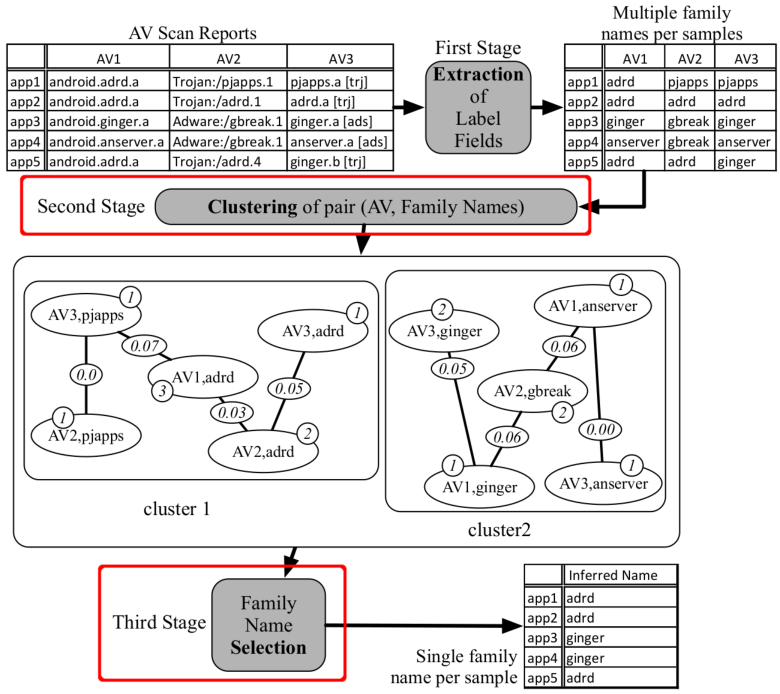
\includegraphics[width=0.8\textwidth]{figures/euphony/architecture-second.pdf}
    \end{figure}

\end{frame}

\begin{frame}
    \frametitle{Stage 2 and 3: clustering and selection of family names}
    \vspace{-15pt}
    \small

    \begin{equation*}
        W(x, y) = 
        (1 - \frac{|x \cap y|}{\min(|x|, |y|)}) +
        \frac{1}{10} \times (1 - \frac{\min(|x|, |y|)}{\max(|x|, |y|)}) +
        \frac{1}{100} \times (1 - dice(x, y))
    \end{equation*}

    \begin{figure}
        \vspace{-10pt}
        \hspace*{-25pt}
        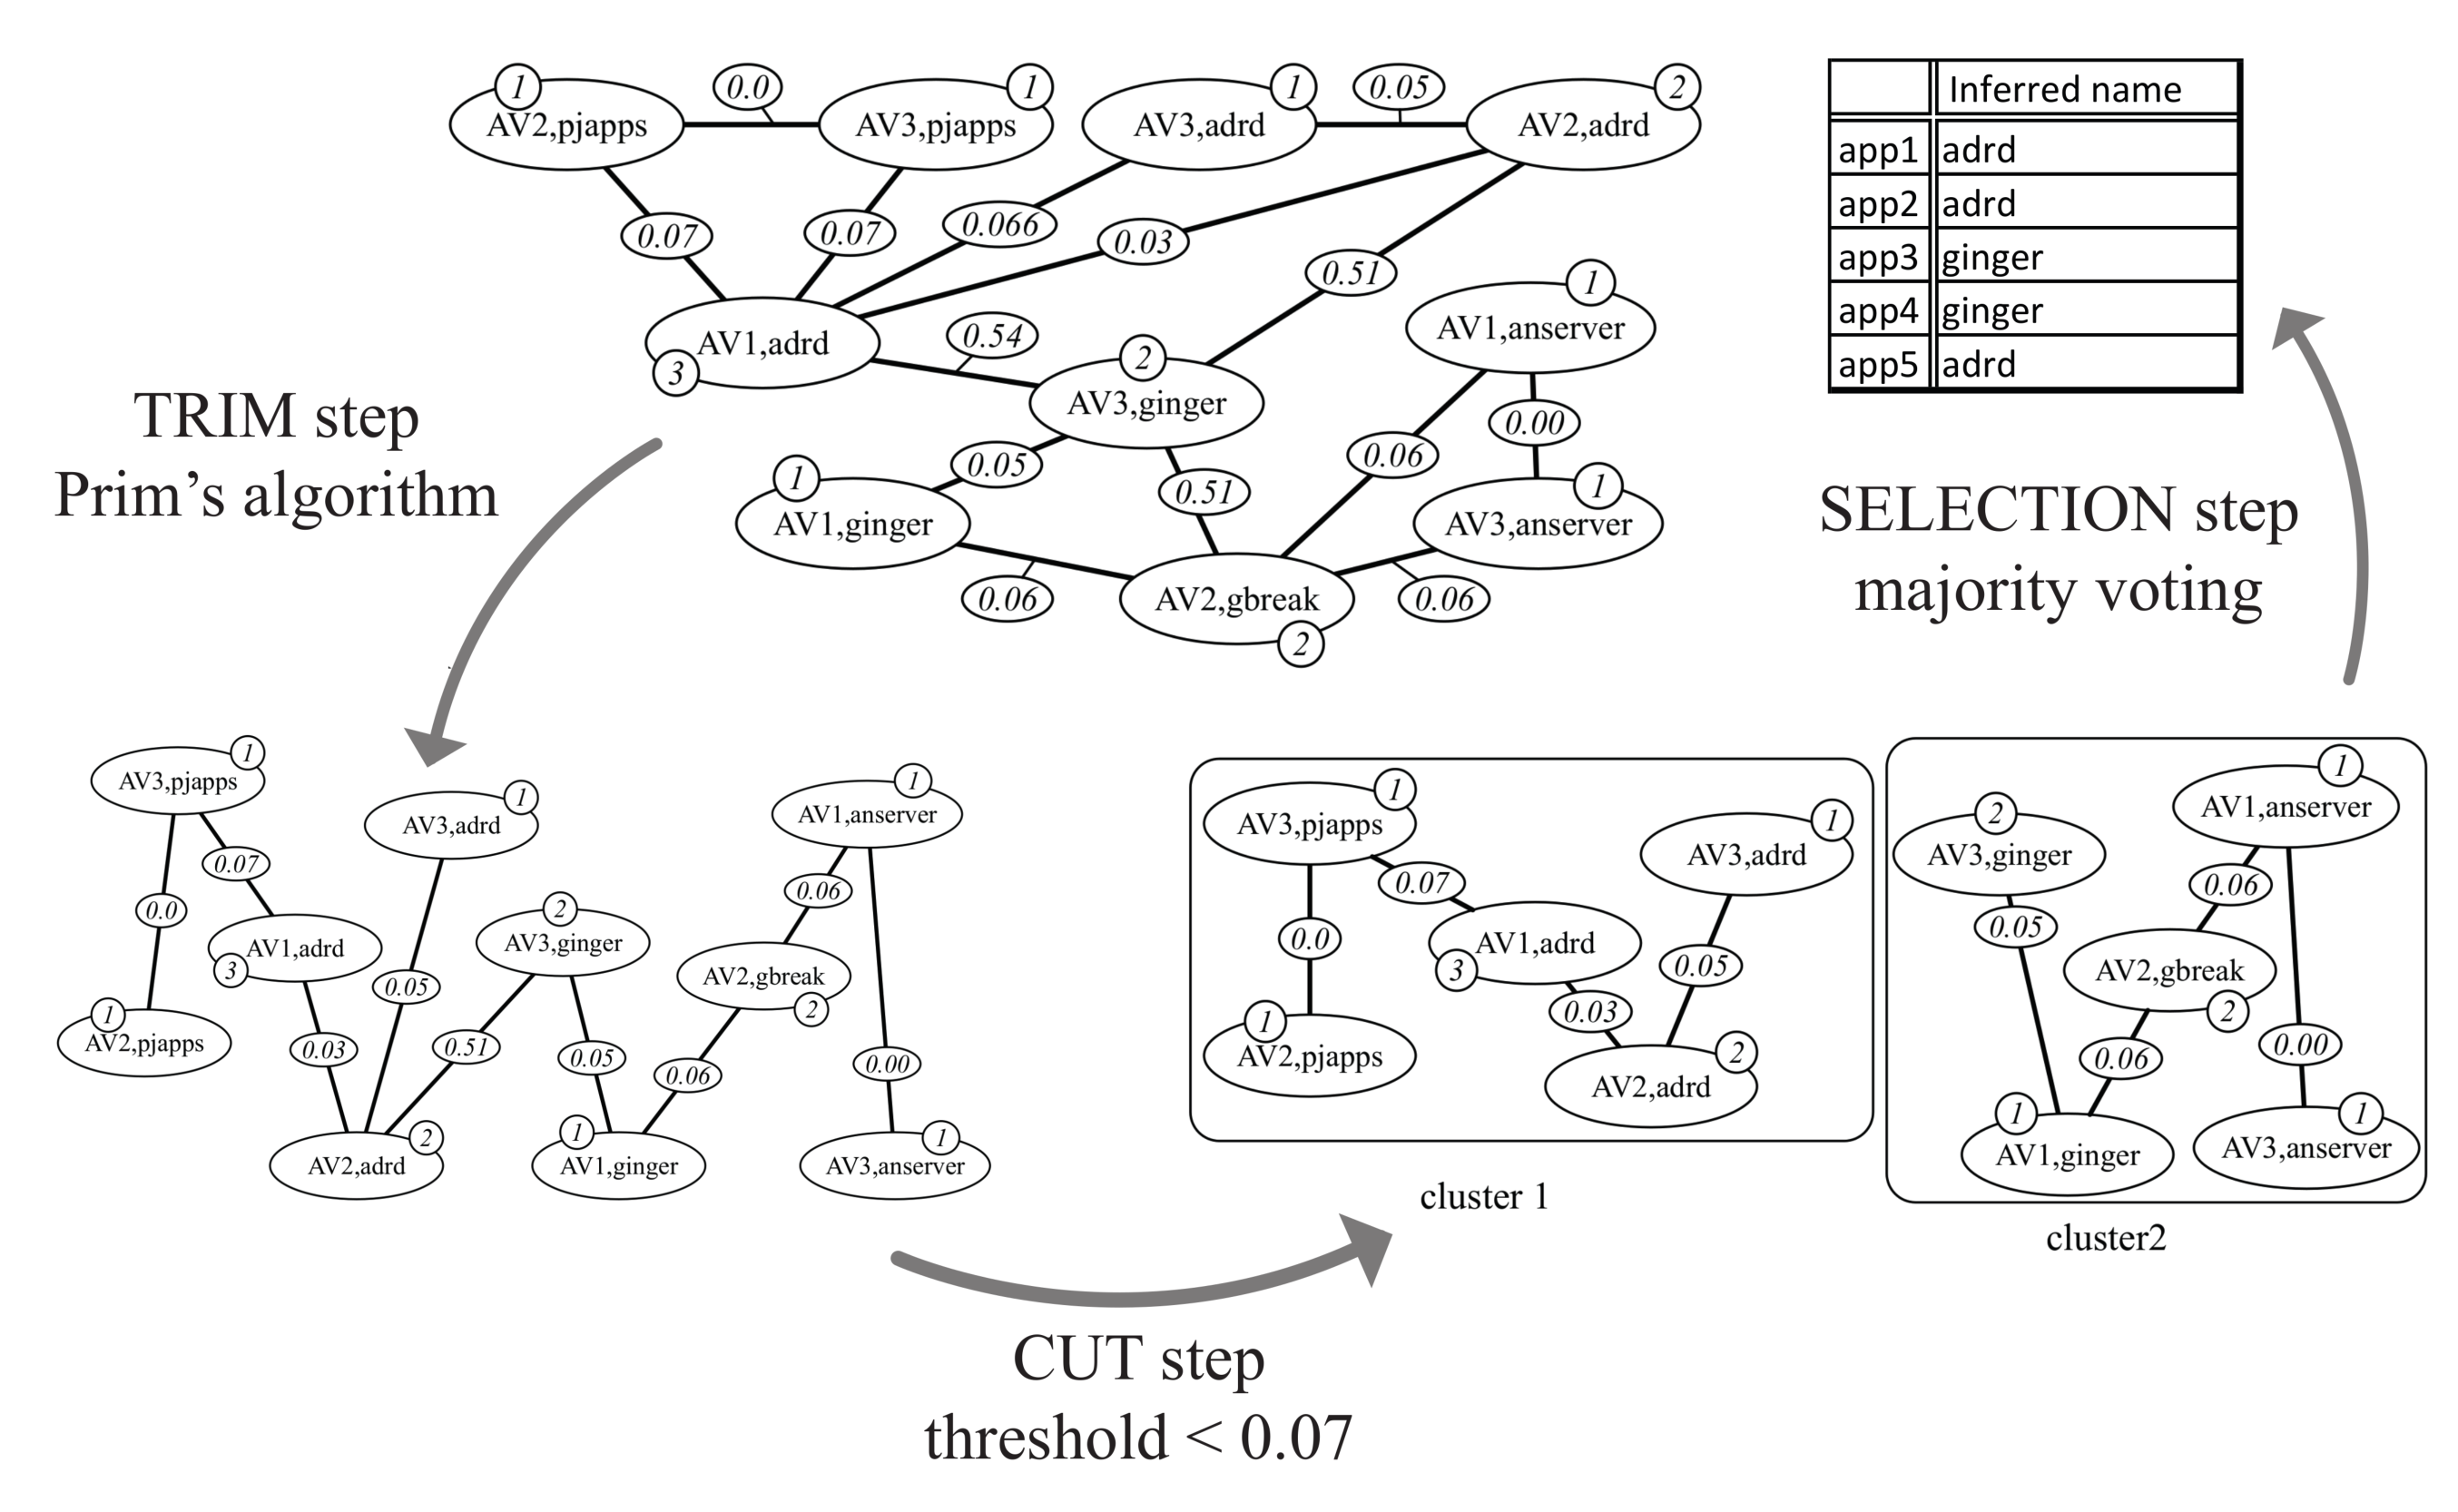
\includegraphics[width=1.05\textwidth]{figures/euphony/clustering.pdf}
    \end{figure}

\end{frame}

\begin{frame}
    \frametitle{Datasets and evaluation against state-of-the-art}
    \centering

    \begin{block}{}
        \centering
        \textbf{Datasets}
    \end{block}
    \smallskip{}
    \begin{table}[!ht]
        \resizebox{0.8\textwidth}{!}{
            \begin{tabular}{|r|r|r|c|}
    \hline
    \textbf{Dataset} & \textbf{\# Samples} & \textbf{\# Families} & \textbf{Collection Period} \\
    \hline
    {\em MalGenome} &  1\,262 & 44 & 2008 - 2010 \\
    {\em Drebin} &  5\,260   & 178 & 2010 - 2012 \\
    {\em Androzoo} & 402\,600 & unknown & 2015 - 2016 \\
    \hline
\end{tabular}

        }
        \caption{\footnotesize{Malware ground truths analyzed for the evaluation of EUPHONY}}
    \end{table}

    \vspace{-15pt}

    \begin{block}{}
        \centering
        \textbf{Evaluation}
    \end{block}
    \smallskip{}
    {\em AVClass} is a labeling tool that outputs the most likely family \\
    \smallskip{}
    It requires a \underline{ground truth} to generate generics and aliases tokens

    \vspace{-10pt}

    \begin{table}
        \resizebox{\textwidth}{!}{
            \begin{tabular}{|c|ccc|ccc|ccc|ccc|}
    \hline
    & \multicolumn{3}{c|}{\textbf{EUPHONY}} & \multicolumn{9}{c|}{{\em \textbf{AVClass}}} \\
    \hline
    & \multicolumn{3}{c|}{-} & \multicolumn{3}{c|}{\textbf{{\em AVClass} Config 1}} & \multicolumn{3}{c|}{\textbf{{\em AVClass} Config 2}} & \multicolumn{3}{c|}{\textbf{{\em AVClass} Config 3}} \\
    & \multicolumn{3}{c|}{- } & \multicolumn{3}{c|}{\em as reported in paper} & \multicolumn{3}{c|}{\em with default files in Git} & \multicolumn{3}{c|}{\em new generics \& aliases} \\
    \hline
    Dataset & Prec & Rec & F1 & Prec & Rec & F1 & Prec & Rec & F1 & Prec & Rec & F1 \\
    \hline
    {\em MalGen.} & 86.7 & 99.7 & \textbf{92.7} & 87.2 & 98.8 & \textbf{92.6} & 86.5 & 98.0 & \textbf{91.9} & 53.9 & 65.2 & \textbf{59.0} \\
    {\em Drebin} & 95.0 & 96.1 & \textbf{95.5} & 95.2 & 92.5 & \textbf{93.9} & 95.4 & 93.0 & \textbf{94.2} & 29.6 & 69.8 & \textbf{41.6} \\
    \hline
\end{tabular}

        }
        \caption{\footnotesize{{Performance of EUPHONY against 3 {\em AVClass} configurations (in \%)}}}
    \end{table}

\end{frame}

\begin{frame}
    \frametitle{Investigation of Androzoo dataset (no ground truth)}
    \centering

    \begin{table}[!ht]
        \resizebox{0.6\textwidth}{!}{
            \begin{tabular}{|c|c|c|c|c|}
    \hline
                        & \textbf{Labeled}  & \textbf{Clusters}   & Singletons & Runtime \\
    \hline
    EUPHONY             & \textbf{319\,100} & \textbf{735}        & 165        & 216s \\
    {\em AVClass}       & \textbf{178\,471} & \textbf{453}        & 135        & 114s \\
    \hline
\end{tabular}

        }
        \caption{\footnotesize{Results of EUPHONY and {\em AVClass} (402~600 samples)}}
    \end{table}

    \vspace{-10pt}

    EUPHONY found more labels and more clusters

    \medskip{}

    \begin{table}[!ht]
        \resizebox{0.65\textwidth}{!}{
            \begin{tabular}{|cr|cr|rr|}
    \hline
    \multicolumn{2}{|c|}{\textbf{EUPHONY}} & \multicolumn{2}{c|}{\textbf{{\em AVClass}}} & \multicolumn{2}{c|}{Intersection} \\
    \hline
    \textbf{Family}    & \textbf{samples} & \textbf{Family}  & \textbf{samples} & samples & overlap (in \%) \\
    \hline
    dowgin    & 33\,297   & dowgin  & 22\,617   & 21\,035   & 93.0 \\
    \textbf{kuguo}     & \textbf{24\,273}   & \textbf{kuguo}   & \textbf{38\,532}   & 24\,072   & 99.2 \\
    secapk    & 17\,889   & secapk  & 20\,492   & 17\,825   & 99.6 \\
    \textbf{addisplay} & \textbf{11\,203}   & \textbf{kuguo}   & \textbf{38\,532}   & 6\,055    & 54.0 \\
    airpush   & 10\,055   & airpush & 13\,202   & 10\,017   & 99.6 \\
    jiagu     & 7\,215    & jiagu   & 8\,987    & 7\,211    & 99.9 \\
    smsreg    & 6\,294    & smsreg  & 8\,427    & 5\,819    & 92.5 \\
    agent     & 6\,088    & feiwo   & 7\,399    & 1\,014    & 16.7 \\
    revmob    & 6\,061    & revmob  & 6\,376    & 6\,058    & 99.9 \\
    generic   & 5\,663    & anydown & 5\,147    & 1\,890    & 36.7 \\
    \hline
\end{tabular}

        }
        \caption{\footnotesize{Top 10 clusters of EUPHONY compared to {\em AVClass}}}
    \end{table}

    \vspace{-11pt}

    EUPHONY clusters seem more granular overall

\end{frame}

\begin{frame}
    \frametitle{Contributions and conclusions}
    \centering

    \begin{block}{}
        \centering
        \textbf{Contributions}
    \end{block}
    \begin{itemize}
        \item Retrieve information from antivirus labels 
        \item Explore relations between antivirus families 
        \item Propose a single family name for experiments 
    \end{itemize}

    \begin{block}{}
        \centering
        \textbf{Conclusions}
    \end{block}
    \begin{itemize}
        \item Information from labels are not sufficient on their own
        \item Malware families provide a guideline for a new approach
        \begin{itemize}
            \item i.e., malware from the same family have the same behaviors
        \end{itemize}
    \end{itemize}

    \vspace{8pt}
    \small{}

    \textbf{How can we reify malicious behaviors from malware families?}

\end{frame}

\begin{frame}
    \frametitle{How to improve the security of Android}

    \begin{tabularx}{\textwidth}{l r}
        \multicolumn{2}{c}{\textbf{Challenge 1:~Definition of Android malware}\vspace{5pt}} \\
        \textbullet~Verify the quality of antivirus results & \textcolor{RED}{STASE} \\
        \textbullet~Retrieve information from antivirus labels & \textcolor{GREEN}{EUPHONY} \\
        \dotline{250pt} & \\
        \\
        \multicolumn{2}{c}{\textbf{Challenge 2:~Detection of Android malware}\vspace{5pt}} \\
        \textbullet~Study the impacts of ground truth settings & \textcolor{RED}{STASE} \\
        \textbullet~Propose a single family name for experiments & \textcolor{GREEN}{EUPHONY} \\
        \dotline{250pt} & \\
        \\
        \multicolumn{2}{c}{\textbf{Challenge 3:~Comprehension of Android malware}\vspace{5pt}} \\
        \textbullet~View the properties of malware ground truths & \textcolor{RED}{STASE} \\
        \textbullet~Explore relations between antivirus families & \textcolor{GREEN}{EUPHONY} \\
        \dotline{250pt} & \\
    \end{tabularx}

\end{frame}
